\begin{figure}
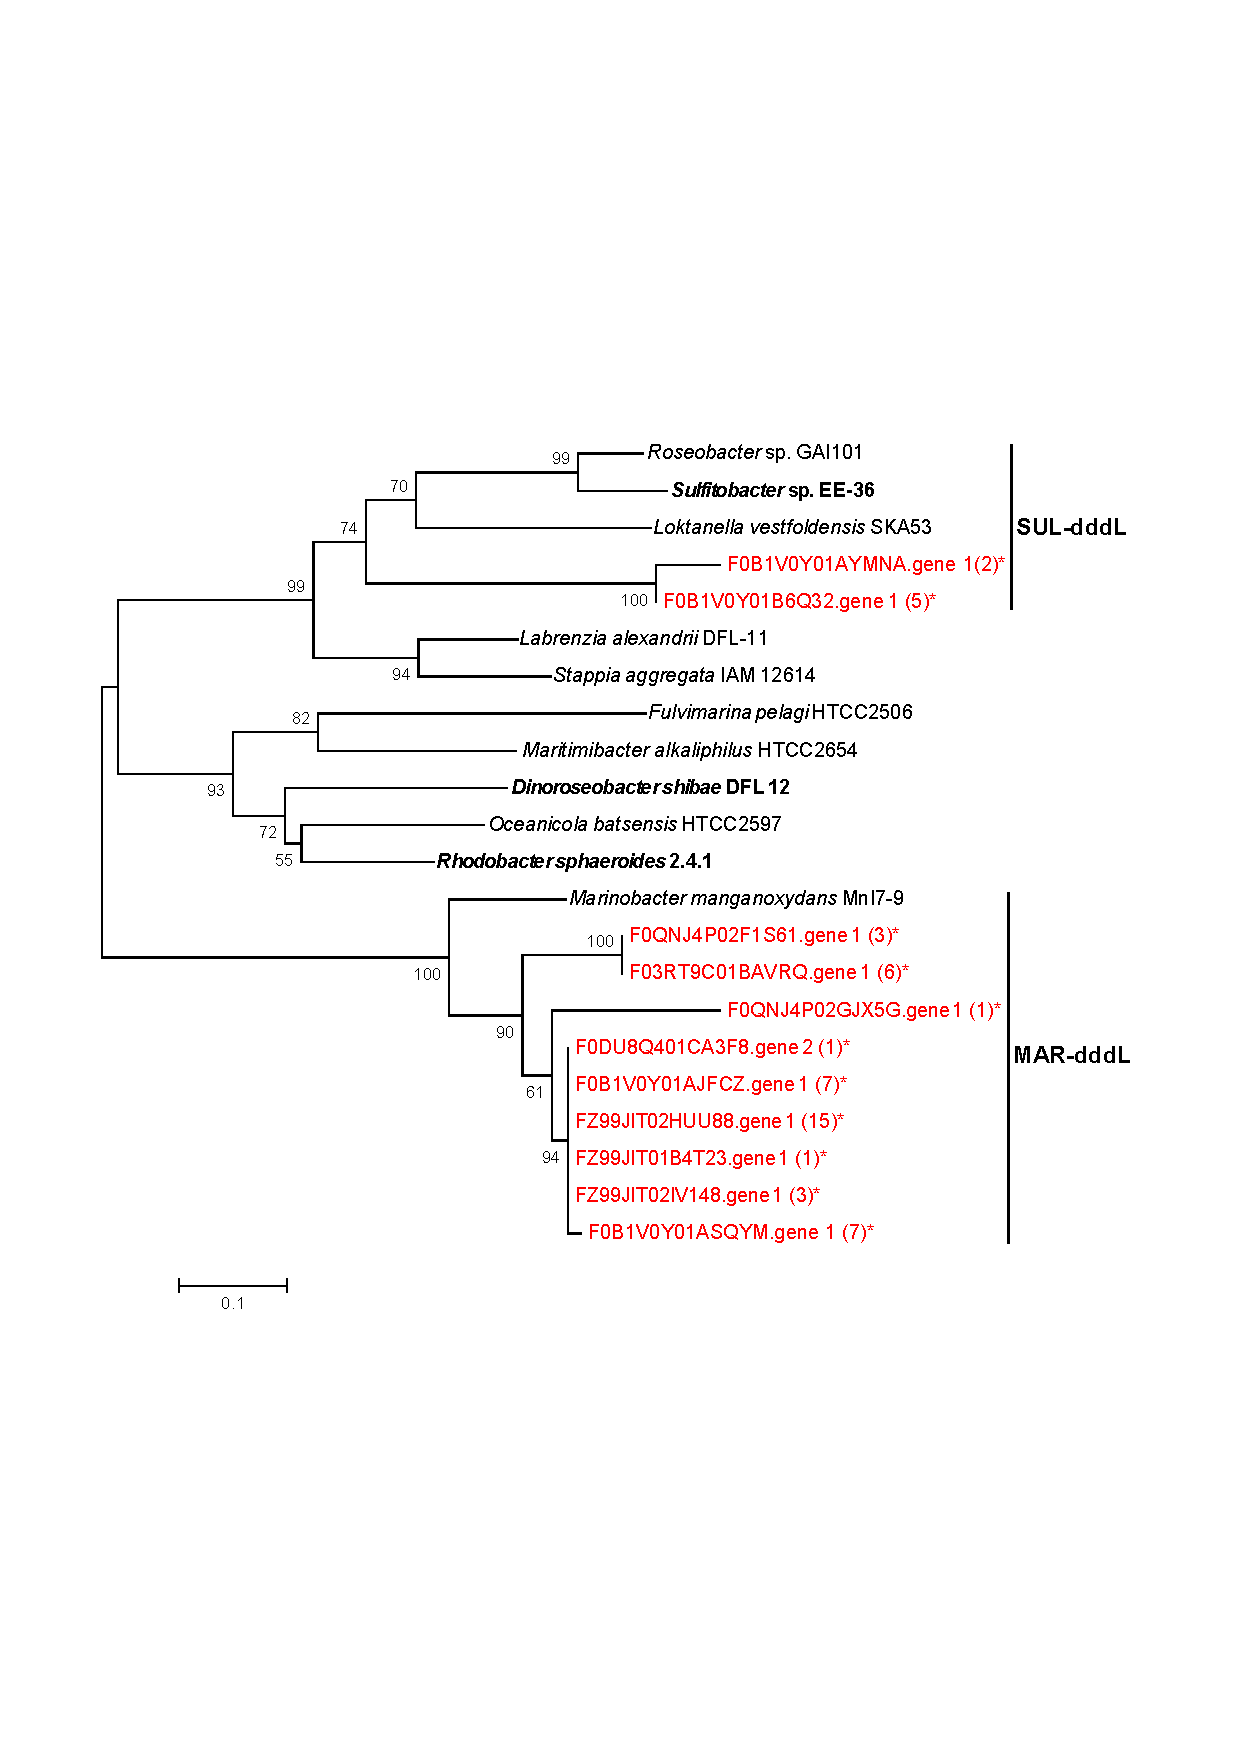
\includegraphics{orglake_figures/dddL_tree.pdf}
\caption[Phylogenetic tree of DddL DMSP lyase homologues]{Phylogenetic tree of DddL DMSP lyase homologues. The tree was computed from an 84 amino acid N-terminal region using the neighbour-joining algorithm. Organic Lake sequences from this study are shown in red and marked with an asterisk (*). Numbers in parentheses are counts of sequences that clustered with the Organic Lake homologue shown in the tree with 90\% amino acid identity. Sequences with confirmed DMSP lyase activity are shown in bold. Accession numbers from top to bottom are: EEB86351, ADK55772, EAQ07081, EEE47811, EAV43167, EAU41122, EAQ10619, ABV95046, EAQ04071, ABA77574 and EHJ04839.}
\label{fig:dddL_tree}

\end{figure}
